\section{Certified Algorithm}

\noindent In this section we initiate the study of certified algorithms for FVS-BCL. We 
begin with a reminder on perturbation resilience and how that is related with the current 
topic. Following that, the next subsection introduces some key concepts that allow us 
to construct certified algorithms in general. Some of them include \textit{m-stitching} 
and the notion of \textit{$\Pi$-m-stitching}. We refer to the literature 
in \cite{bumpus_et_al:LIPIcs.SWAT.2024.19, venne2022designing}. Finally, we construct 
a certified algorithm for FVS-BCL.

\noindent Unless specified otherwise, let $\Pi$ be a vertex-minimization problem.

\subsection{Perturbation resilience}

\subsection{\textit{m-stitching} and \textit{$\Pi$-m-stitching}}

\noindent As we mentioned before, in this section we refer to Bumpus et al. \cite{bumpus_et_al:LIPIcs.SWAT.2024.19} 
and a Master's thesis on the subject by Venne \cite{venne2022designing} with more examples. 

\noindent The restriction we imposed on the Feedback Vertex Set problem enables us to look 
for optimal solutions in a local space. This is what m-stitching and \textit{$\Pi$-m-stitching}
hint at. Here, the the variable $m$ is a positive integer that depends on the vertex optimization 
problem $\Pi$ at hand. In our case this is tied to the $\rho$ argument, i. e. the length of 
the cycles we are trying to break. 

\noindent To introduce \textit{$\Pi$-m-stitching}, one needs to first understand m-stitching and m-stitchable problems. In the stitching 
operation we are given solutions $S_1$ and $S_2$ for a vertex optimization problem, 
along with an induced subgraph $J$ of $G$. Intuitively, we take the portion of $S_1$, that is not a part 
of $J$ and "stitch" onto it some part of $S_2$ along the subgraph $J$. 

\noindent The formal definition is as follows:

\refstepcounter{definition}
\begin{mydefinition}[m-stitching]{Def.}
    \label{m-stitch}

    Assume $m \geq 0$ is an integer, $J$ is an induced subgraph of $G$, and 
    $S_1, S_2 \subseteq V(G)$. Then we define the \textit{m-stitch} of $S_2$ onto $S_1$ along 
    $J$ as the set:

    \[S_3 := (S_1 \backslash V(J)) \cup (S_2 \cap N^{m}_{G} \left[V(J)\right]).\]

\end{mydefinition}

\begin{figure}[H]
    \centering
    \begin{minipage}{0.50\textwidth}
        \centering
        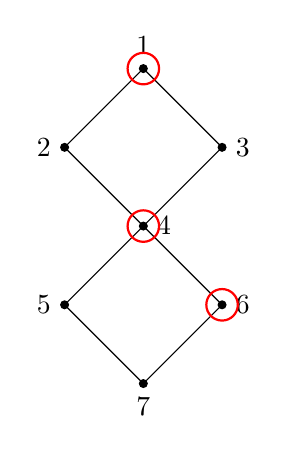
\begin{tikzpicture}
            % Define nodes
            \node[draw, circle, fill=black, scale=0.3, label=above:1] (1) at (0,2) {};
            \node[draw, circle, fill=black, scale=0.3, label=left:2] (2) at (-1,1) {};
            \node[draw, circle, fill=black, scale=0.3, label=right:3] (3) at (1,1) {};
            \node[draw, circle, fill=black, scale=0.3, label=right:4] (4) at (0,0) {};
            \node[draw, circle, fill=black, scale=0.3, label=left:5] (5) at (-1,-1) {};
            \node[draw, circle, fill=black, scale=0.3, label=right:6] (6) at (1,-1) {};
            \node[draw, circle, fill=black, scale=0.3, label=below:7] (7) at (0,-2) {};

            % Draw edges
            \draw (1) -- (2);
            \draw (1) -- (3);
            \draw (2) -- (4);
            \draw (3) -- (4);
            \draw (4) -- (5);
            \draw (4) -- (6);
            \draw (5) -- (7);
            \draw (6) -- (7);


            \draw[red, thick] (1) circle(0.2);
            \draw[red, thick] (4) circle(0.2);
            \draw[red, thick] (6) circle(0.2);

        \end{tikzpicture}
        \caption{Vertex set $S_1$}
    \end{minipage}
    \hfill
    \begin{minipage}{0.49\textwidth}
        \centering
        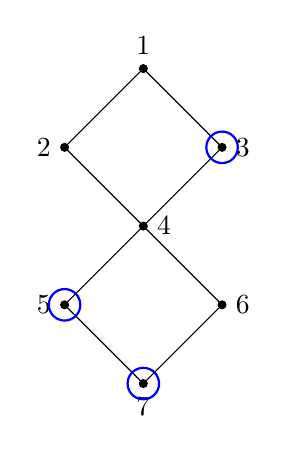
\begin{tikzpicture}
            % Define nodes
            \node[draw, circle, fill=black, scale=0.3, label=above:1] (1) at (0,2) {};
            \node[draw, circle, fill=black, scale=0.3, label=left:2] (2) at (-1,1) {};
            \node[draw, circle, fill=black, scale=0.3, label=right:3] (3) at (1,1) {};
            \node[draw, circle, fill=black, scale=0.3, label=right:4] (4) at (0,0) {};
            \node[draw, circle, fill=black, scale=0.3, label=left:5] (5) at (-1,-1) {};
            \node[draw, circle, fill=black, scale=0.3, label=right:6] (6) at (1,-1) {};
            \node[draw, circle, fill=black, scale=0.3, label=below:7] (7) at (0,-2) {};

            % Draw edges
            \draw (1) -- (2);
            \draw (1) -- (3);
            \draw (2) -- (4);
            \draw (3) -- (4);
            \draw (4) -- (5);
            \draw (4) -- (6);
            \draw (5) -- (7);
            \draw (6) -- (7);

            \draw[blue, thick] (3) circle(0.2);
            \draw[blue, thick] (5) circle(0.2);
            \draw[blue, thick] (7) circle(0.2);

        \end{tikzpicture}
        \caption{Vertex set $S_2$}
    \end{minipage}
\end{figure}

\noindent In the following we show the subgraph $J$ we have chosen and the 2-neighbourhood 
of the subgraph.

\noindent Also, in Fig.~\ref{fig:remove_s1} we show the first step of the m-stitch operation, namely 
removing the vertices of $J$ from the set $S_1$.

\begin{figure}[H]
    \centering
    \begin{minipage}{0.50\textwidth}
        \centering
        \begin{tikzpicture}
            % Define nodes
            \node[draw, circle, fill=black, scale=0.3, label=above:1] (1) at (0,2) {};
            \node[draw, circle, fill=black, scale=0.3, label=left:2] (2) at (-1,1) {};
            \node[draw, circle, fill=black, scale=0.3, label=right:3] (3) at (1,1) {};
            \node[draw, circle, fill=black, scale=0.3, label=right:4] (4) at (0,0) {};
            \node[draw, circle, fill=black, scale=0.3, label=left:5] (5) at (-1,-1) {};
            \node[draw, circle, fill=black, scale=0.3, label=right:6] (6) at (1,-1) {};
            \node[draw, circle, fill=black, scale=0.3, label=below:7] (7) at (0,-2) {};

            % Draw edges
            \draw (1) -- (2);
            \draw (1) -- (3);
            \draw (2) -- (4);
            \draw (3) -- (4);
            \draw (4) -- (5);
            \draw (4) -- (6);
            \draw (5) -- (7);
            \draw (6) -- (7);

            \begin{scope}[on background layer]
                \filldraw[orange!70,line width=20pt,rounded corners=5pt] (2.center) -- (3.center) -- (6.center) -- (7.center) -- (5.center) -- cycle;
            \end{scope}

            \begin{scope}[on background layer]   
                \filldraw[orange!35,line width=20pt,rounded corners=5pt] (6.center) --  (7.center) -- cycle;
            \end{scope}

        \end{tikzpicture}
        \caption{Subgraph $J$ of $G$ in light orange and $N^{2}_{G}\left[V(J)\right]$ in darker orange}
    \end{minipage}
    \hfill
    \begin{minipage}{0.49\textwidth}
        \centering
        \begin{tikzpicture}
            % Define nodes
            \node[draw, circle, fill=black, scale=0.3, label=above:1] (1) at (0,2) {};
            \node[draw, circle, fill=black, scale=0.3, label=left:2] (2) at (-1,1) {};
            \node[draw, circle, fill=black, scale=0.3, label=right:3] (3) at (1,1) {};
            \node[draw, circle, fill=black, scale=0.3, label=right:4] (4) at (0,0) {};
            \node[draw, circle, fill=black, scale=0.3, label=left:5] (5) at (-1,-1) {};
            \node[draw, circle, fill=black, scale=0.3, label=right:6] (6) at (1,-1) {};
            \node[draw, circle, fill=black, scale=0.3, label=below:7] (7) at (0,-2) {};

            % Draw edges
            \draw (1) -- (2);
            \draw (1) -- (3);
            \draw (2) -- (4);
            \draw (3) -- (4);
            \draw (4) -- (5);
            \draw (4) -- (6);
            \draw (5) -- (7);
            \draw (6) -- (7);

            \begin{scope}[on background layer]   
                \filldraw[orange!70,line width=20pt,rounded corners=5pt] (2.center) -- (3.center) -- (6.center) -- (7.center) -- (5.center) -- cycle;
            \end{scope}

            \begin{scope}[on background layer]   
                \filldraw[orange!35,line width=20pt,rounded corners=5pt] (6.center) --  (7.center) -- cycle;
            \end{scope}

            \draw[red, thick] (1) circle(0.2);
            \draw[red, thick] (4) circle(0.2);

        \end{tikzpicture}
        \caption{Remove $V(J)$ from $S_1$}
        \label{fig:remove_s1}
    \end{minipage}
\end{figure}

\noindent What follows is the second step in obtaining set $S_3$ in Fig.~\ref{fig:second_step} and the 
stitched set in Fig.~\ref{fig:stitched_set}.

\begin{figure}[H]
    \centering
    \begin{minipage}{0.50\textwidth}
        \centering
        \begin{tikzpicture}
            % Define nodes
            \node[draw, circle, fill=black, scale=0.3, label=above:1] (1) at (0,2) {};
            \node[draw, circle, fill=black, scale=0.3, label=left:2] (2) at (-1,1) {};
            \node[draw, circle, fill=black, scale=0.3, label=right:3] (3) at (1,1) {};
            \node[draw, circle, fill=black, scale=0.3, label=right:4] (4) at (0,0) {};
            \node[draw, circle, fill=black, scale=0.3, label=left:5] (5) at (-1,-1) {};
            \node[draw, circle, fill=black, scale=0.3, label=right:6] (6) at (1,-1) {};
            \node[draw, circle, fill=black, scale=0.3, label=below:7] (7) at (0,-2) {};

            % Draw edges
            \draw (1) -- (2);
            \draw (1) -- (3);
            \draw (2) -- (4);
            \draw (3) -- (4);
            \draw (4) -- (5);
            \draw (4) -- (6);
            \draw (5) -- (7);
            \draw (6) -- (7);

            \begin{scope}[on background layer]   
                \filldraw[orange!70,line width=20pt,rounded corners=5pt] (2.center) -- (3.center) -- (6.center) -- (7.center) -- (5.center) -- cycle;
            \end{scope}

            \begin{scope}[on background layer]   
                \filldraw[orange!35,line width=20pt,rounded corners=5pt] (6.center) --  (7.center) -- cycle;
            \end{scope}

            \draw[red, thick] (1) circle(0.2);
            \draw[red, thick] (4) circle(0.2);

            \draw[blue, thick] (3) circle(0.2);
            \draw[blue, thick] (5) circle(0.2);
            \draw[blue, thick] (7) circle(0.2);


        \end{tikzpicture}
        \caption{Add $S_2 \cap N^{2}_{G} \left[V(J)\right]$}
        \label{fig:second_step}
    \end{minipage}
    \hfill
    \begin{minipage}{0.49\textwidth}
        \centering
        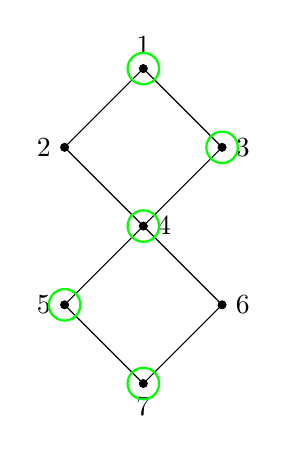
\begin{tikzpicture}
            % Define nodes
            \node[draw, circle, fill=black, scale=0.3, label=above:1] (1) at (0,2) {};
            \node[draw, circle, fill=black, scale=0.3, label=left:2] (2) at (-1,1) {};
            \node[draw, circle, fill=black, scale=0.3, label=right:3] (3) at (1,1) {};
            \node[draw, circle, fill=black, scale=0.3, label=right:4] (4) at (0,0) {};
            \node[draw, circle, fill=black, scale=0.3, label=left:5] (5) at (-1,-1) {};
            \node[draw, circle, fill=black, scale=0.3, label=right:6] (6) at (1,-1) {};
            \node[draw, circle, fill=black, scale=0.3, label=below:7] (7) at (0,-2) {};

            % Draw edges
            \draw (1) -- (2);
            \draw (1) -- (3);
            \draw (2) -- (4);
            \draw (3) -- (4);
            \draw (4) -- (5);
            \draw (4) -- (6);
            \draw (5) -- (7);
            \draw (6) -- (7);

            \draw[green, thick] (1) circle(0.2);
            \draw[green, thick] (3) circle(0.2);
            \draw[green, thick] (4) circle(0.2);
            \draw[green, thick] (5) circle(0.2);
            \draw[green, thick] (7) circle(0.2);

        \end{tikzpicture}
        \caption{Set $S_3$}
        \label{fig:stitched_set}
    \end{minipage}
\end{figure}

\noindent A problem $\Pi$ is \textit{m-stitchable} if the set of feasible solutions are closed 
under the m-stitching operator. We hope that when we take the union in \ref{m-stitch} and arrive 
at the set $S_3$, this would too be a feasible solution.

\refstepcounter{definition}
\begin{mydefinition}[m-stitchable]{Def.}
    \label{m-stitchable}

    For an integer $m \geq 0$, induced subgraph $J$ and feasible solutions $S_1, S_2 \subseteq V(G)$ 
    of a vertex optimization problem $\Pi$ we have that the m-stitching of $S_2$ onto $S_1$ along 
    $J$, $S_3$ is a feasible solution to $\Pi$ on $G$.

\end{mydefinition}

\noindent Now that we have a definition for problems $\Pi$ that are m-stitchable, we introduce 
$\Pi$-m-stitching as defined in \cite{bumpus_et_al:LIPIcs.SWAT.2024.19} and afterwards apply 
it to the current problem.

\refstepcounter{definition}
\begin{mydefinition}[$\Pi$-m-stitching]{Algorithm.}
    \label{p-m-stitching}

    \textbf{Input:}
    an instance ($G, w : V(G) \to \mathbb{N}$) to an m-stitchable vertex optimization problem $\Pi$ 
    along with a solution $S$ and a vertex set $J \subseteq V(G)$.

    \textbf{Task:}
    find a feasible solution $S^{\prime}$ to $\Pi$ on $G$, such that for all other feasible solutions 
    $S^*$ it holds that $w(S^{\prime}) \leq w\left(\text{m-stitch}(S^{*}, S)\right)$.

\end{mydefinition}

\noindent Before we proceed with the main theorem that we use to construct a certified algorithm 
we need one more definition.

\refstepcounter{definition}
\begin{mydefinition}[Guessable]{Def.}
    \label{guessable}

    \noindent A problem $\Pi$ is guessable if there is an algorithm that outputs a feasible solution 
    with no requirement for optimality in polynomial time.

\end{mydefinition}

The following is Theorem 1.7 in \cite{bumpus_et_al:LIPIcs.SWAT.2024.19}.

\refstepcounter{definition}
\begin{mydefinition}[Theorem 1.7 in \cite{bumpus_et_al:LIPIcs.SWAT.2024.19}]{Theorem.}
    \label{theorem-main}

    Let $\mathbb{G}$ be a minor-closed graph class whose local tree-width is bounded above by a linear 
    function of the form $g : r \to \lambda \cdot r$ (fixed $\lambda \in \mathbb{R}$ and $r \in \mathbb{N}$).
    If $\Pi$ is a vertex-minimization problem and it holds that:

    \begin{enumerate}
        \item $\Pi$ is guessable.
        \item $\Pi$ is m-stitchable.
        \item There exists an algorithm $A_{\Pi}$ which solves $\Pi$-m-stitching in time $f(t) \cdot  |V(G)|^{\mathbb{O}(1)}$,
        where t = \textbf{tw}($G\left[N^{m}_{G}(J)\right]$) and $f$ is a computable function;
        then, for each $\epsilon > 0$ there is a $(1 + \epsilon)$-certified algorithm for $\Pi$ that 
        runs in time $f(\lambda \cdot m / \epsilon) \cdot \left|V(G)\right| ^ {\mathbb{O}(1)}$.
    \end{enumerate}

\end{mydefinition}

\subsection{Certified Algorithm}

\noindent The proof of theorem \ref{theorem-main} is beyond the scope of this paper. In this section 
we only apply the three steps, mentioned to the FVS-BCL problem without generalizing to other 
vertex-minimization problems. 

\noindent Firstly, we take a look at the guessable property.

\refstepcounter{definition}
\begin{mydefinition}[FVS-BCL is guessable]{Lemma}
    \label{lemma-guessable}

    \noindent For any planar graph $G$, the set $V(G)$ is a feasible solution to FVS-BCL.

\end{mydefinition}

\noindent \textit{Proof}. The set $V(G)$ trivially satisfies the fact that every 4-cycle would be broken.

\refstepcounter{definition}
\begin{mydefinition}[FVS-BCL is 2-stitchable]{Lemma}
    \label{lemma-m-stitchable}

    \noindent Let $(G, w)$ be any instance to the FVS-BCL problem, $J \subseteq G$ any induced subgraph 
    and $S_1$ and $S_2$ any two feasible solutions to the problem in $G$. It suffices to prove that 
    $S_3$ is a feasible solution, where: 
    \[S_3 := (S_1 \backslash V(J)) \cup (S_2 \cap N^{2}_{G} \left[V(J)\right]).\]

    Let any 4-cycle be of vertices $v_1, v_2, v_3, v_4$.

\end{mydefinition}

\noindent \textit{Proof}. We inspect the possible cases for the 4-cycle $v_1 v_2 v_3 v_4$. In order 
to prove \ref{lemma-m-stitchable} we have to prove that there exists a $v \in \{v_1, v_2, v_3, v_4\}$,
such that $v \in S_3$. 

\begin{enumerate}[label=\textbf{•}]
    \item $\exists v^{\prime} \in \{v_1,v_2,v_3,v_4\}$, such that $v^{\prime} \in J$.

    Now we can argue for the vertex $v$. Because one of the vertices of the cycle in question is in 
    $J$, then we can argue that one of them will be in the intersection $S_2 \cap N^{2}_{G}[V(J)]$. 
    Formally,

    \begin{enumerate}
        \item Because $v^{\prime} \in J$, no vertex $v'' \in V(G) \backslash N^{2}_{G}[V(J)]$ can be 
        a part of the set $v_1,v_2,v_3,v_4$ and therefore break the cycle.
        \item However, $S_2$ is a feasible solution and in that intersection $S_2 \cap N^{2}_{G}[V(J)]$ 
        it follows that $\exists v \in N^{2}_{G}[V(J)]$, such that $v \in \{v_1,v_2,v_3,v_4\}$.
        \item Finally, $S_2 \cap N^{2}_{G}[V(J)] \subseteq S_3$, therefore $v \in S_3$.
    \end{enumerate}

    \item $\forall v' \in \{v_1,v_2,v_3,v_4\}$, it holds that $v' \notin J$. This case is simpler 
    as it follows from the feasibility of $S_1$. This is because the operation $S_1 \backslash V(J)$ 
    would not remove any vertex $v'$ from the cycle. What also holds is that $S_1 \backslash V(J) \subseteq S_3$. 
    Finally, we piece together the fact that for $v \in \{v_1,v_2,v_3,v_4\}$ it holds that 
    $v \in S_3$.

\end{enumerate}